
%% bare_conf.tex
%% V1.3
%% 2007/01/11
%% by Michael Shell
%% See:
%% http://www.michaelshell.org/
%% for current contact information.
%%
%% This is a skeleton file demonstrating the use of IEEEtran.cls
%% (requires IEEEtran.cls version 1.7 or later) with an IEEE conference paper.
%%
%% Support sites:
%% http://www.michaelshell.org/tex/ieeetran/
%% http://www.ctan.org/tex-archive/macros/latex/contrib/IEEEtran/
%% and
%% http://www.ieee.org/

%%*************************************************************************
%% Legal Notice:
%% This code is offered as-is without any warranty either expressed or
%% implied; without even the implied warranty of MERCHANTABILITY or
%% FITNESS FOR A PARTICULAR PURPOSE! 
%% User assumes all risk.
%% In no event shall IEEE or any contributor to this code be liable for
%% any damages or losses, including, but not limited to, incidental,
%% consequential, or any other damages, resulting from the use or misuse
%% of any information contained here.
%%
%% All comments are the opinions of their respective authors and are not
%% necessarily endorsed by the IEEE.
%%
%% This work is distributed under the LaTeX Project Public License (LPPL)
%% ( http://www.latex-project.org/ ) version 1.3, and may be freely used,
%% distributed and modified. A copy of the LPPL, version 1.3, is included
%% in the base LaTeX documentation of all distributions of LaTeX released
%% 2003/12/01 or later.
%% Retain all contribution notices and credits.
%% ** Modified files should be clearly indicated as such, including  **
%% ** renaming them and changing author support contact information. **
%%
%% File list of work: IEEEtran.cls, IEEEtran_HOWTO.pdf, bare_adv.tex,
%%                    bare_conf.tex, bare_jrnl.tex, bare_jrnl_compsoc.tex
%%*************************************************************************

% *** Authors should verify (and, if needed, correct) their LaTeX system  ***
% *** with the testflow diagnostic prior to trusting their LaTeX platform ***
% *** with production work. IEEE's font choices can trigger bugs that do  ***
% *** not appear when using other class files.                            ***
% The testflow support page is at:
% http://www.michaelshell.org/tex/testflow/



% Note that the a4paper option is mainly intended so that authors in
% countries using A4 can easily print to A4 and see how their papers will
% look in print - the typesetting of the document will not typically be
% affected with changes in paper size (but the bottom and side margins will).
% Use the testflow package mentioned above to verify correct handling of
% both paper sizes by the user's LaTeX system.
%
% Also note that the "draftcls" or "draftclsnofoot", not "draft", option
% should be used if it is desired that the figures are to be displayed in
% draft mode.
%
\documentclass[10pt, conference, compsocconf]{IEEEtran}
% Add the compsocconf option for Computer Society conferences.
%
% If IEEEtran.cls has not been installed into the LaTeX system files,
% manually specify the path to it like:
% \documentclass[conference]{../sty/IEEEtran}


\newcommand{\TODO}{\textbf{TODO:} }


% Some very useful LaTeX packages include:
% (uncomment the ones you want to load)


% *** MISC UTILITY PACKAGES ***
%
%\usepackage{ifpdf}
% Heiko Oberdiek's ifpdf.sty is very useful if you need conditional
% compilation based on whether the output is pdf or dvi.
% usage:
% \ifpdf
%   % pdf code
% \else
%   % dvi code
% \fi
% The latest version of ifpdf.sty can be obtained from:
% http://www.ctan.org/tex-archive/macros/latex/contrib/oberdiek/
% Also, note that IEEEtran.cls V1.7 and later provides a builtin
% \ifCLASSINFOpdf conditional that works the same way.
% When switching from latex to pdflatex and vice-versa, the compiler may
% have to be run twice to clear warning/error messages.






% *** CITATION PACKAGES ***
%
%\usepackage{cite}
% cite.sty was written by Donald Arseneau
% V1.6 and later of IEEEtran pre-defines the format of the cite.sty package
% \cite{} output to follow that of IEEE. Loading the cite package will
% result in citation numbers being automatically sorted and properly
% "compressed/ranged". e.g., [1], [9], [2], [7], [5], [6] without using
% cite.sty will become [1], [2], [5]--[7], [9] using cite.sty. cite.sty's
% \cite will automatically add leading space, if needed. Use cite.sty's
% noadjust option (cite.sty V3.8 and later) if you want to turn this off.
% cite.sty is already installed on most LaTeX systems. Be sure and use
% version 4.0 (2003-05-27) and later if using hyperref.sty. cite.sty does
% not currently provide for hyperlinked citations.
% The latest version can be obtained at:
% http://www.ctan.org/tex-archive/macros/latex/contrib/cite/
% The documentation is contained in the cite.sty file itself.






% *** GRAPHICS RELATED PACKAGES ***
%
\ifCLASSINFOpdf
  \usepackage[pdftex]{graphicx}
  % declare the path(s) where your graphic files are
  % \graphicspath{{../pdf/}{../jpeg/}}
  % and their extensions so you won't have to specify these with
  % every instance of \includegraphics
  % \DeclareGraphicsExtensions{.pdf,.jpeg,.png}
\else
  % or other class option (dvipsone, dvipdf, if not using dvips). graphicx
  % will default to the driver specified in the system graphics.cfg if no
  % driver is specified.
  % \usepackage[dvips]{graphicx}
  % declare the path(s) where your graphic files are
  % \graphicspath{{../eps/}}
  % and their extensions so you won't have to specify these with
  % every instance of \includegraphics
  % \DeclareGraphicsExtensions{.eps}
\fi
% graphicx was written by David Carlisle and Sebastian Rahtz. It is
% required if you want graphics, photos, etc. graphicx.sty is already
% installed on most LaTeX systems. The latest version and documentation can
% be obtained at: 
% http://www.ctan.org/tex-archive/macros/latex/required/graphics/
% Another good source of documentation is "Using Imported Graphics in
% LaTeX2e" by Keith Reckdahl which can be found as epslatex.ps or
% epslatex.pdf at: http://www.ctan.org/tex-archive/info/
%
% latex, and pdflatex in dvi mode, support graphics in encapsulated
% postscript (.eps) format. pdflatex in pdf mode supports graphics
% in .pdf, .jpeg, .png and .mps (metapost) formats. Users should ensure
% that all non-photo figures use a vector format (.eps, .pdf, .mps) and
% not a bitmapped formats (.jpeg, .png). IEEE frowns on bitmapped formats
% which can result in "jaggedy"/blurry rendering of lines and letters as
% well as large increases in file sizes.
%
% You can find documentation about the pdfTeX application at:
% http://www.tug.org/applications/pdftex





% *** MATH PACKAGES ***
%
%\usepackage[cmex10]{amsmath}
% A popular package from the American Mathematical Society that provides
% many useful and powerful commands for dealing with mathematics. If using
% it, be sure to load this package with the cmex10 option to ensure that
% only type 1 fonts will utilized at all point sizes. Without this option,
% it is possible that some math symbols, particularly those within
% footnotes, will be rendered in bitmap form which will result in a
% document that can not be IEEE Xplore compliant!
%
% Also, note that the amsmath package sets \interdisplaylinepenalty to 10000
% thus preventing page breaks from occurring within multiline equations. Use:
%\interdisplaylinepenalty=2500
% after loading amsmath to restore such page breaks as IEEEtran.cls normally
% does. amsmath.sty is already installed on most LaTeX systems. The latest
% version and documentation can be obtained at:
% http://www.ctan.org/tex-archive/macros/latex/required/amslatex/math/





% *** SPECIALIZED LIST PACKAGES ***
%
%\usepackage{algorithmic}
% algorithmic.sty was written by Peter Williams and Rogerio Brito.
% This package provides an algorithmic environment fo describing algorithms.
% You can use the algorithmic environment in-text or within a figure
% environment to provide for a floating algorithm. Do NOT use the algorithm
% floating environment provided by algorithm.sty (by the same authors) or
% algorithm2e.sty (by Christophe Fiorio) as IEEE does not use dedicated
% algorithm float types and packages that provide these will not provide
% correct IEEE style captions. The latest version and documentation of
% algorithmic.sty can be obtained at:
% http://www.ctan.org/tex-archive/macros/latex/contrib/algorithms/
% There is also a support site at:
% http://algorithms.berlios.de/index.html
% Also of interest may be the (relatively newer and more customizable)
% algorithmicx.sty package by Szasz Janos:
% http://www.ctan.org/tex-archive/macros/latex/contrib/algorithmicx/




% *** ALIGNMENT PACKAGES ***
%
%\usepackage{array}
% Frank Mittelbach's and David Carlisle's array.sty patches and improves
% the standard LaTeX2e array and tabular environments to provide better
% appearance and additional user controls. As the default LaTeX2e table
% generation code is lacking to the point of almost being broken with
% respect to the quality of the end results, all users are strongly
% advised to use an enhanced (at the very least that provided by array.sty)
% set of table tools. array.sty is already installed on most systems. The
% latest version and documentation can be obtained at:
% http://www.ctan.org/tex-archive/macros/latex/required/tools/


%\usepackage{mdwmath}
%\usepackage{mdwtab}
% Also highly recommended is Mark Wooding's extremely powerful MDW tools,
% especially mdwmath.sty and mdwtab.sty which are used to format equations
% and tables, respectively. The MDWtools set is already installed on most
% LaTeX systems. The lastest version and documentation is available at:
% http://www.ctan.org/tex-archive/macros/latex/contrib/mdwtools/


% IEEEtran contains the IEEEeqnarray family of commands that can be used to
% generate multiline equations as well as matrices, tables, etc., of high
% quality.


%\usepackage{eqparbox}
% Also of notable interest is Scott Pakin's eqparbox package for creating
% (automatically sized) equal width boxes - aka "natural width parboxes".
% Available at:
% http://www.ctan.org/tex-archive/macros/latex/contrib/eqparbox/





% *** SUBFIGURE PACKAGES ***
\usepackage[tight,footnotesize]{subfigure}
% subfigure.sty was written by Steven Douglas Cochran. This package makes it
% easy to put subfigures in your figures. e.g., "Figure 1a and 1b". For IEEE
% work, it is a good idea to load it with the tight package option to reduce
% the amount of white space around the subfigures. subfigure.sty is already
% installed on most LaTeX systems. The latest version and documentation can
% be obtained at:
% http://www.ctan.org/tex-archive/obsolete/macros/latex/contrib/subfigure/
% subfigure.sty has been superceeded by subfig.sty.



%\usepackage[caption=false]{caption}
%\usepackage[font=footnotesize]{subfig}
% subfig.sty, also written by Steven Douglas Cochran, is the modern
% replacement for subfigure.sty. However, subfig.sty requires and
% automatically loads Axel Sommerfeldt's caption.sty which will override
% IEEEtran.cls handling of captions and this will result in nonIEEE style
% figure/table captions. To prevent this problem, be sure and preload
% caption.sty with its "caption=false" package option. This is will preserve
% IEEEtran.cls handing of captions. Version 1.3 (2005/06/28) and later 
% (recommended due to many improvements over 1.2) of subfig.sty supports
% the caption=false option directly:
%\usepackage[caption=false,font=footnotesize]{subfig}
%
% The latest version and documentation can be obtained at:
% http://www.ctan.org/tex-archive/macros/latex/contrib/subfig/
% The latest version and documentation of caption.sty can be obtained at:
% http://www.ctan.org/tex-archive/macros/latex/contrib/caption/




% *** FLOAT PACKAGES ***
%
%\usepackage{fixltx2e}
% fixltx2e, the successor to the earlier fix2col.sty, was written by
% Frank Mittelbach and David Carlisle. This package corrects a few problems
% in the LaTeX2e kernel, the most notable of which is that in current
% LaTeX2e releases, the ordering of single and double column floats is not
% guaranteed to be preserved. Thus, an unpatched LaTeX2e can allow a
% single column figure to be placed prior to an earlier double column
% figure. The latest version and documentation can be found at:
% http://www.ctan.org/tex-archive/macros/latex/base/



%\usepackage{stfloats}
% stfloats.sty was written by Sigitas Tolusis. This package gives LaTeX2e
% the ability to do double column floats at the bottom of the page as well
% as the top. (e.g., "\begin{figure*}[!b]" is not normally possible in
% LaTeX2e). It also provides a command:
%\fnbelowfloat
% to enable the placement of footnotes below bottom floats (the standard
% LaTeX2e kernel puts them above bottom floats). This is an invasive package
% which rewrites many portions of the LaTeX2e float routines. It may not work
% with other packages that modify the LaTeX2e float routines. The latest
% version and documentation can be obtained at:
% http://www.ctan.org/tex-archive/macros/latex/contrib/sttools/
% Documentation is contained in the stfloats.sty comments as well as in the
% presfull.pdf file. Do not use the stfloats baselinefloat ability as IEEE
% does not allow \baselineskip to stretch. Authors submitting work to the
% IEEE should note that IEEE rarely uses double column equations and
% that authors should try to avoid such use. Do not be tempted to use the
% cuted.sty or midfloat.sty packages (also by Sigitas Tolusis) as IEEE does
% not format its papers in such ways.





% *** PDF, URL AND HYPERLINK PACKAGES ***
%
\usepackage[allowmove]{url}
% url.sty was written by Donald Arseneau. It provides better support for
% handling and breaking URLs. url.sty is already installed on most LaTeX
% systems. The latest version can be obtained at:
% http://www.ctan.org/tex-archive/macros/latex/contrib/misc/
% Read the url.sty source comments for usage information. Basically,
% \url{my_url_here}.



\usepackage{multirow}

% *** Do not adjust lengths that control margins, column widths, etc. ***
% *** Do not use packages that alter fonts (such as pslatex).         ***
% There should be no need to do such things with IEEEtran.cls V1.6 and later.
% (Unless specifically asked to do so by the journal or conference you plan
% to submit to, of course. )


% correct bad hyphenation here
\hyphenation{op-tical net-works semi-conduc-tor}

% avoid orphans and widows
\clubpenalty = 10000
\widowpenalty = 10000
\displaywidowpenalty = 10000

%
\usepackage{flushend} 

\begin{document}
%
% paper title
% can use linebreaks \\ within to get better formatting as desired
% \title{Verification of Bug Fixes: What Does it Really Mean?}
\title{Characterizing Verification of Bug Fixes in Two Open Source IDEs}


% author names and affiliations
% use a multiple column layout for up to two different
% affiliations

\author{
\IEEEauthorblockN{Rodrigo Souza and Christina Chavez}
\IEEEauthorblockA{Software Engineering Labs\\
Department of Computer Science - IM\\
Universidade Federal da Bahia (UFBA), Brazil \\
\{rodrigo,flach\}@dcc.ufba.br}
}

% conference papers do not typically use \thanks and this command
% is locked out in conference mode. If really needed, such as for
% the acknowledgment of grants, issue a \IEEEoverridecommandlockouts
% after \documentclass

% for over three affiliations, or if they all won't fit within the width
% of the page, use this alternative format:
% 
%\author{\IEEEauthorblockN{Michael Shell\IEEEauthorrefmark{1},
%Homer Simpson\IEEEauthorrefmark{2},
%James Kirk\IEEEauthorrefmark{3}, 
%Montgomery Scott\IEEEauthorrefmark{3} and
%Eldon Tyrell\IEEEauthorrefmark{4}}
%\IEEEauthorblockA{\IEEEauthorrefmark{1}School of Electrical and Computer Engineering\\
%Georgia Institute of Technology,
%Atlanta, Georgia 30332--0250\\ Email: see http://www.michaelshell.org/contact.html}
%\IEEEauthorblockA{\IEEEauthorrefmark{2}Twentieth Century Fox, Springfield, USA\\
%Email: homer@thesimpsons.com}
%\IEEEauthorblockA{\IEEEauthorrefmark{3}Starfleet Academy, San Francisco, California 96678-2391\\
%Telephone: (800) 555--1212, Fax: (888) 555--1212}
%\IEEEauthorblockA{\IEEEauthorrefmark{4}Tyrell Inc., 123 Replicant Street, Los Angeles, California 90210--4321}}




% use for special paper notices
%\IEEEspecialpapernotice{(Invited Paper)}




% make the title area
\maketitle

% how verification is actually performed and reported on specific software projects.

\begin{abstract}
	Data from bug repositories have been used to enable inquiries about software product and process quality. Unfortunately, such repositories often contain inaccurate, inconsistent, or missing data, which can originate misleading results. 
	% In this paper, we show how data from bug repositories can be mined in order to give insights about the process of software verification in two open source projects, Eclipse and NetBeans.
	In this paper, we investigate how well data from bug repositories support the discovery of details about the software verification process in two open source projects, Eclipse and NetBeans.
	%In this paper, we investigate the process of verification of bug fixes of two open source projects, Eclipse and NetBeans, by analyzing only the data in bug repositories. 
	We have been able do identify quality assurance teams in NetBeans and to detect a well-defined verification phase in Eclipse. 
	A major challenge, however, was to identify the verification techniques used in the projects. Moreover, we found cases in which a large batch of bug fixes is simultaneously reported to be verified, although no software verification was actually done. 
	Such mass verifications, if not acknowledged, threatens analyses that rely on information about software verification reported on bug repositories. Therefore, we recommend that the exploratory analyses presented in this paper precede inferences based on reported verifications. %on bug reports.
	% Knowing details from the verification process of a project and how it is reported on bug repositories is valuable to anyone interested in studying software verification using a data-based approach. 
	% 
	% Such pitfalls for data analyses should be taken into account in any future research relying on verification information from bug repositories
	% 
	% Future research should take into 
	% pitfalls of data.
	%  account such threats when analyzing 
	% It is recommended
	% 
	% Also, we found periods in which a large batch of bug fixes is marked 
	% 
	% In this paper, we investigate the reported status of bug reports from the projects Eclipse and Netbeans, in special the VERIFIED status, corresponding to the verification that a  bug fix is appropriate. We show that the VERIFIED status is used in a variety of distinct ways, not always consistent with the traditional definition of software verification.
	% Future research should take into account the multiple contexts in which the VERIFIED status is used when deriving conclusions based on the data from bug reports.
\end{abstract}

\begin{IEEEkeywords}
mining software repositories; bug tracking systems; software verification; empirical study.
\end{IEEEkeywords}

% For peer review papers, you can put extra information on the cover
% page as needed:
% \ifCLASSOPTIONpeerreview
% \begin{center} \bfseries EDICS Category: 3-BBND \end{center}
% \fi
%
% For peerreview papers, this IEEEtran command inserts a page break and
% creates the second title. It will be ignored for other modes.
\IEEEpeerreviewmaketitle

% http://wiki.eclipse.org/Development_Resources/HOWTO/Bugzilla_Use
%   The severity tags aren't used much, except to distinguish enhancements from bugs. Typically the users specify severities as they see fit.

% http://wiki.eclipse.org/Bug_Reporting_FAQ
%   when a test pass comes up a component owner can build a query that searched for resolved bugs
%   After testing that the fix worked a resolved bug can be transitioned to verified, directly to closed, or in fact, reopened. 
%   By searching for bugs with a Status of verified and a resolution of fixed developers can come up with release notes.
%   Severity is assigned by a user and describes the level of impact the bug is having on them. Priority is assigned by the developer and describes the importance a developer places on fixing the bug.

\newcommand{\UNCONFIRMED}{\texttt{UNCONFIRMED}}
\newcommand{\NEW}{\texttt{NEW}}
\newcommand{\ASSIGNED}{\texttt{ASSIGNED}}
\newcommand{\VERIFIED}{\texttt{VERIFIED}}
\newcommand{\RESOLVED}{\texttt{RESOLVED}}
\newcommand{\CLOSED}{\texttt{CLOSED}}
\newcommand{\REOPENED}{\texttt{REOPENED}}
\newcommand{\FIXED}{\texttt{FIXED}}

\begin{section}{Introduction}

Bug repositories have for a long time been used in software projects to support coordination among stakeholders. They record discussion and progress of software evolution activities, such as bug fixing and software verification. Hence, bug repositories are an opportunity for researchers who intend to investigate issues related to the quality of both the product and the process of a software development team.
%, or even issues regarding the nature of software development itself.

% The information contained in bug repositories has been used in order to predict fault-proneness, to unveil developers' roles from data, to characterize transfer of work in software projects, and so on. Also, it has been used to investigate beliefs in software engineering related to software quality, such as the impact of developer turnover and of collective ownership on the occurrence of bugs.

However, mining bug repositories has its own risks. Previous research has identified problems of missing data (e.g., rationale, traceability links between reported bug fixes and source code changes) and inaccurate data (e.g., misclassification of bugs) \cite{Aranda2009}. %,Bird2009,Nguyen2010,Ayari2007}.

  In previous research \cite{Souza2011}, we tried to assess the impact of independent verification of bug fixes on software quality, by mining data from bug repositories. 
  We relied on reported verifications tasks, as recorded in bug reports, and interpreted the recorded data according to the documentation for the specific bug tracking system used.
  As the partial results suggested that verification has no impact on software quality, we questioned the accuracy of the data about verification of bug fixes, and thus decided to investigate how verification is actually performed and reported on the projects that were analyzed, Eclipse and NetBeans.
	
	Hence, in this paper, we investigate the following exploratory research questions regarding the software verification process in Eclipse and NetBeans:

	\begin{itemize}
		\item \textbf{How} is the verification performed: are there performed ad hoc tests, automated tests, code inspection?
		\item \textbf{Who} performs the verification: is there a QA (quality assurance) team? 
		\item \textbf{When} is the verification performed: is it performed just after the fix, or is there a verification phase?
		% \item How is the distribution of verification across developers?
		% \item Is there a dedicated team for QA?
	\end{itemize}

	The next section contains some background information about bug tracking systems and software verification. In Section \ref{sec:methods}, the data and methods used to investigate the research questions are presented. Then, in Section \ref{sec:results}, the results are exposed and discussed. Finally, Section \ref{sec:conclusion} presents some concluding remarks.

% In summary, for researchers who intend to use data from bug tracking systems, it is not sufficient to understand the data fields in a bug report the way they are documented in the system's documentation. The research should also investigate whether the data fields are used often, whether they are used accordingly to the documentation, and even if the data fields are used consistently across the developers.

% In this paper, we investigate the status of a bug, a data field present in most bug tracking systems that reports the progress of the bug solving activity. In particular, we focus on the activity of verification of a fix. We are interested in answering the following exploratory research questions:

% For research question xx, qualitative of a small sample. 
% For research question xx, all bugs were considered.

\end{section}

\begin{section}{Background} \label{sec:background}
% Bug workflow. Bugzilla. \cite{Bird2009}

% Reposit ́orios de bugs. Arquivam relat ́orios de defeitos e solicitac ̧ ̃oes de mudan ̧ca. Tais reposito ́rios ajudam os desenvolvedores a registrar, discutir e acompanhar a situa ̧ca ̃o de cada solicita ̧c ̃ao, desde a atribui ̧ca ̃o de uma solicita ̧ca ̃o a um desenvolvedor at ́e a verifica ̧c ̃ao da corre ̧c ̃ao ou melhoria. Exemplos incluem o Bugzilla, o Trac e o Jira.

Bug tracking systems allow users and developers of a software project to manage a list of bugs for the project, along with information such as steps to reproduce the bug, its severity and the operating system used. Developers choose bugs to fix and can report on the progress of the bug fixing activities, ask for clarification, discuss causes for the bug etc.

In this research, we focus on Bugzilla, an open source bug tracking system used by notable software projects such as Eclipse, Mozilla, Linux Kernel, NetBeans, Apache, and companies such as NASA and Facebook\footnote{Complete list available at http://www.bugzilla.org/installation-list/.}. The general concepts from Bugzilla should apply to most other bug tracking systems.

One important feature of a bug that is recorded on bug tracking systems is its status. The status records the progress of the bug fixing activity.
%, and, as such, provides data to software engineering studies
Figure \ref{fig:bugzilla} shows each status that can be recorded in Bugzilla, along with typical transitions between status values, i.e., the workflow.

\begin{figure}[ht]
	\centering
		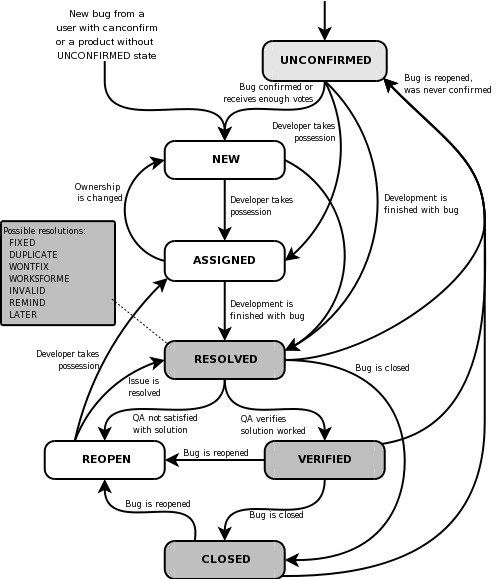
\includegraphics[scale=0.4]{bugzilla.png}
	\caption{Workflow for Bugzilla. Source: \url{http://www.bugzilla.org/docs/2.18/html/lifecycle.html}.}
	\label{fig:bugzilla}
\end{figure}

In the simplest cases, a bug is created and receive the status \UNCONFIRMED\ (if it was created by a regular user) or \NEW\ (if it was created by a developer). Next, it is \ASSIGNED\ to a developer, and then it is \RESOLVED, possibly by fixing it with a patch on the source code. The solution is then \VERIFIED\ by someone in the quality assurance team, if it is adequate, or otherwise it is \REOPENED. When a version of the software is released, all \VERIFIED\ bugs are \CLOSED.

% If it passes the quality requirements, it is \CLOSED\ when the next release of the software is released. If it does not pass the quality requirements or if the solution only partially fixes the problem, the bug is \REOPENED.

% Roles: reporter, fixer, verifier, reopener, closer.

% bugs with status \VERIFIED\ are used to write the release notes / change log.

% In order to understand the bug fixing process of a software team, however, it should be possible to know what activities are performed upon change of status. 
%For example, what steps are made before changing the status of a bug to RESOLVED (FIXED)? Is the patch applied to the version control system? Is it presented as diff file attached to the bug report? Is there a build available to end users containing the patch (e.g., a nightly build)? The documentation for Bugzilla does not prescribe specific activities for marking a bug as RESOLVED, relegating instead this decision to each software project.
%
%Similarly, w
%What do developers do before marking a bug as \VERIFIED? 
Bugzilla documentation states that, when a bug is \VERIFIED, it means that ``QA [quality assurance team] has looked at the bug and the resolution and agrees that the appropriate resolution has been taken''\footnote{\url{https://landfill.bugzilla.org/bugzilla-3.6-branch/page.cgi?id=fields.html}}. It does not specify how developers should look at the resolution (e.g., by looking at the source code, or by running a patched version of the software). 

% Again, the definition is broad, although it assumes the existence of a QA team.

% The developer documentation for both Eclipse and NetBeans are unclear about how the verification of a bug fix is performed. So, what are the forms of software verification used in the verification process of these projects?

% In some parts they mention running unit tests, and running a patched version of the software and try to reproduce the bug.

Software verification techniques are classified in static and dynamic \cite{Sommerville1995}. Static techniques include \emph{source code inspection}, automated \emph{static analysis}, and \emph{formal verification}. Dynamic techniques, or testing, involve executing the software system under certain conditions and comparing its actual behavior with the intended behavior. Testing can be done in an improvised way (\emph{ad hoc testing}), or it can be structured as a list of test cases, leading to \emph{automated testing}.

% While mining bug repositories, one cannot assume that the \VERIFIED\ status comprises all forms of software verification. Also, one cannot rely on the information provided by the bug tracking system or the developer documentation for a project, since it can be too generic to be useful. Such information can be assessed by taking a closer look on actual bug reports.

% O bug não se manifesta após a aplicação da solução.
% A solução não gera novos bugs.
% O código da solução segue as convenções de codificação e políticas do projeto.
% A solução possui uma boa relação custo-benefício — isto é, ou não existem soluções melhores ou a solução é um paliativo por conta da alta complexidade de uma solução melhor.
% 
% Minha expectativa, portanto, é que, antes de o bug ser marcado como VERIFICADO, ele passe pelas seguintes atividades:
% 
% Aplicação do patch com a solução do bug na versão do software onde o bug foi encontrado.
% Execução do software com o bug, seguindo os passos para reprodução do bug, e verificando que o bug não se manifesta
% Inspeção do código-fonte. Deve ser verificada a aderência às convenções de codificação do projeto e a outras políticas (por exemplo, cada patch deve vir com testes de unidade).
% Execução de testes de unidade (se houver). Deve se verificar que todos os testes passam.

\end{section}

\begin{section}{Method} \label{sec:methods}

	% \item How is the verification actually performed?
	% \item When is the verification performed (i.e., just after the fix, or is there a specific period for the verification of fixed bugs?)
	% \item Who performs the verification?

	In order to answer the research questions---when and how bug fixes are verified, and who verifies them---, a three-part method was used:
	
	\begin{enumerate}
		\item \textbf{Data extraction}: we have obtained publicly available raw data from the Bugzilla repositories of two popular integrated development environments, Eclipse and NetBeans.

		\item \textbf{Data sampling}: for each project, two representative subprojects were chosen for analysis.
		
		% we have chosen two subprojects. After that, we sampled bugs with interesting characteristics.
		
		% \item \textbf{Informal analysis}: some bug reports were fully read, so insights could be gained from them.
		
		\item \textbf{Data analysis}: for each research question, a distinct analysis was required. The analyses will be further described.
	\end{enumerate}	
	
	The experimental package is available at \url{https://sites.google.com/site/rodrigorgs2/msr2012}.

\begin{subsection}{Data Extraction}
	
	In order to perform the desired analyses, we needed access to the data recorded by Bugzilla for a specific project, including status changes and comments. We have found such data for two projects---Eclipse and NetBeans---from the domain of integrated development environments. The data were made available as part of the Mining Software Repositories 2011 Challenge\footnote{\url{http://www.msrconf.org/msr-challenge.html}} in the form of MySQL database dumps. The files contain all data from the respective databases, except for developer profiles, omitted for privacy reasons.
	
	% We have had access to Eclipse Bugzilla database from October, 2001 to June, 2010, and to NetBeans Bugzilla database from ... to .... The data was made available as part of the Mining Software Repositories 2011 Challenge\footnote{\url{http://www.msrconf.org/msr-challenge.html}} as a SQL dump. The SQL dump contains all information recorded by Bugzilla for the projects (except for information about developers, which was removed for privacy reasons).

	Eclipse development began in late 1998 with IBM\footnote{\url{http://www.ibm.com/developerworks/rational/library/nov05/cernosek/}}. It was licensed as open source in November, 2001. The available data set contains 316,911 bug reports for its 155 subprojects, from October, 2001 to June, 2010.
		
	NetBeans\footnote{\url{http://netbeans.org/about/history.html}} started  as a student project in 1996. It was then bought by Sun Microsystems in October, 1999, and open sourced in March, 2000. The data set contains 185,578 bug reports for its 39 subprojects, from June, 1998 to June, 2010.
	
\end{subsection}

\begin{subsection}{Data Sampling}

	Four subprojects were chosen for further analysis: Eclipse/Platform, Eclipse/EMF, NetBeans/Platform, and NetBeans/VersionControl. The Platform subprojects are the main subprojects for the respective IDEs, so they are both important and representative of each projects' philosophy. 
	
	The other two subprojects were chosen at random, restricted to subprojects in which the proportion of verified bugs was greater than the proportion observed in the respective Platform subprojects. The reason is to avoid selecting projects in which bugs are seldom marked as \VERIFIED. The following proportions of \VERIFIED\ bugs per project were observed: Eclipse/Platform: 16.0\%; Eclipse/EMF: 48.4\%; NetBeans/Platform: 21.4\%; NetBeans/VersionControl: 29.7\%.
	
	% NetBeans/VersionControl: 0.29694479
	% NetBeans/Platform: 0.21423101
	% Eclipse/EMF: 0.4835361489
	% Eclipse/Platform: 0.1595397738
	
	% In order to obtain insight about the research questions, we read a sample of bug reports from both projects. For each project, two subprojects were chosen randomly among the projects with most verified bugs, resulting in the following subprojects: Eclipse/Platform, Eclipse/EMF, NetBeans/platform, NetBeans/versioncontrol. We have sampled 20 bug reports for each subproject, totalizing 80 bug reports.
	% 
	
\end{subsection}

\begin{subsection}{Analysis: How Are Bugs Verified?}

	In order to discover the verification techniques used by the subprojects, we have looked at the comments written by developers when they mark a bug as \VERIFIED\ (meaning that the fix was accepted) or \REOPENED\ (meaning that the fix was rejected). First, an informal analysis was performed, by reading a sample of such comments, looking for textual patterns that indicate that a particular technique was used. Then, based on the informal analysis and on previous knowledge, a regular expression was built for each technique, to match comments in which there is evidence that that particular technique was used. The regular expressions were refined by looking at the results matched by them and modifying them to avoid false positives. 
	
	The complete regular expressions are available in the experimental package. For the sake of simplicity, the following list describes only some substrings matched by the regular expressions for each technique:
		
	\begin{itemize}
		\item automated testing: testcase, test case, unit test, automated test, test result, run the test, test run;
		\item source code inspection: inspecting, inspection, look at the code, looking at the source;
		\item ad hoc testing: verified by running, verified by [word ending in ``ing''];
		\item automated static analysis: findbugs, checkstyle, static code, static analys;
		\item formal testing: formal test, formal verif.
	\end{itemize}
	
	% The classification script is smart enough to ignore negative assertions, such as ``did not run the test''.	
	
	During the informal analysis, it was observed that ad hoc testing is reported in many distinct ways that are difficult to capture by means of regular expressions. Hence, its regular expression is expected to match only a few comments.
	
	% The regular expression for ad hoc testing is the most restrictive of them, because ad hoc testing was found to be reported in many distinct ways (when it is reported). %We expect to find fewer examples of ad hoc testing than it should be found.
	
\end{subsection}

\begin{subsection}{Analysis: When Are Bugs Verified?}
	
	In order to determine if there is a well-defined verification phase for the subprojects, we have selected all reported verifications (i.e., status changes to \VERIFIED) over the lifetime of each subproject. Then, we have plotted, for each day in the interval, the accumulated number of verifications reported since the first day available in the data. The curve is monotonically increasing, with steeper ascents representing periods of intense verification activity.
	
	Also, we have obtained the release dates for multiple versions of Eclipse and NetBeans. The information was obtained in the respective websites. In cases in which older information was not available, archived versions of the web pages were accessed via the website \url{www.archive.org}.
	
	If a subproject presents a well-defined verification phase, it is expected that the verification activity is more intense a few days before a release. Such pattern can be identified by visual inspection of the graph, by looking for steeper ascents in the verification curve preceding the release dates.
	
\end{subsection}

\begin{subsection}{Analysis: Who Verifies Bugs?}
	
	In order to determine whether there is a team dedicated to quality assurance (QA), we have counted how many times each developer has marked a bug as \FIXED\ or \VERIFIED. We considered that a developer is part of a QA team if s/he verified at least 10 times (i.e., one order of magnitude) more than s/he fixed bugs. Also, we have computed the proportion of verifications that was performed by the discovered QA team. It is expected that, if the discovered set of developers is actually a QA team, they should be responsible for the majority of the verifications.
	
\end{subsection}

\end{section}

\begin{section}{Results and Discussion} \label{sec:results}
	
	Each of the three analysis was performed on Eclipse/Platform, Eclipse/EMF, NetBeans/Platform, and NetBeans/VersionControl. The results are presented next.
	
% \begin{subsection}{Preliminary Analysis}
% 	Some insights were gained in this step, partially answering the who, when, and how questions:
% 	
% 	\begin{itemize}
% 		\item [how] (OK) In some projects, the status VERIFIED does not correspond to software verification. In Eclipse/EMF, for example, it means that the fix is available in a build that is promoted on the project website\footnote{\url{http://wiki.eclipse.org/Modeling_PMC_Meeting,_2007-10-16} (between releases 3.3.1 and 3.3.1.1)}. Further evidence: bug #254489 ``Please do not change the state of the bugs since the status verified fixed should be only there when we publish a new build. :-)''
% 		\item [(who)] (NOT RELEVANT) In the NetBeans subprojects that were analyzed, it was common that the reporter also verified the fix. In some bugs, this was necessary since the developer was not able to reproduce the bug.
% 		\item [(who, when)] Often, the fixer verifies the bug just after marking it as fixed.
% 		\item [(when)] (OK) Sometimes, several old bugs are marked as VERIFIED at the same time.
% 		\item [(how?)] (OK) In both Eclipse and NetBeans, it is common that the fixer requests someone else to verify the fix (``Please verify, Tom'').
% 		\item [(how)] (OK) In Eclipse/EMF, bug #249436, one developer rewrites the patch submitted by other developer.
% 		\item [(how)] (OK) In Eclipse/EMF, bug #269789, a test case is used to assess the proposed fix.
% 		\item [(how)] (OK) Eclipse/Platform, bug #210533: ``Verified by code inspection''.
% 	\end{itemize}
% 	
% \end{subsection}	
	
\begin{subsection}{How Are Bugs Verified?}

  % To identify the verification techniques used by the projects, we looked at messages written by developers when they mark a bug as VERIFIED (meaning that the bug fix is appropriate) or REOPENED (meaning that some problem was found in the proposed fix). First, we have read some messages, non-systematically, to get some idea of what is said in theses messages and how it is said.

	Table \ref{tab:how} shows, for each subproject, the number of comments associated with a bug being marked as \VERIFIED\ or \REOPENED\ that refers to a particular verification technique. No references to formal verification or static analysis were found; therefore, these techniques are not shown on the table.

	\begin{table}
		\begin{center}
		\caption{Verification techniques for all four subprojects.}
		\begin{tabular}{l|r|r|r}
			% \toprule
			\textbf{\centering Project} & 
			\textbf{\centering Testing} & 
			\textbf{\centering Inspection} & 
			\textbf{\centering Ad Hoc} \\
			\hline
			Eclipse/Platform        & 260 (1.1\%) & 524 (2.2\%) & 74 (0.3\%) \\
			Eclipse/EMF             & 27 (0.7\%) & 2 (0.1\%) & 0 (0.0\%) \\
			NetBeans/Platform       & 94 (0.6\%) & 5 (0.0\%) & 0 (0.0\%) \\
			NetBeans/VersionControl & 4 (0.1\%) & 1 (0.0\%) & 0 (0.0\%) 
			% \bottomrule
		\end{tabular}
		\end{center}
		
		\label{tab:how}
	\end{table}

	In Eclipse/Platform, less than 4\% of the comments referenced the verification technique that was used; for the other projects, less than 1\% of the comments contained such references. Such low proportion reveals how difficult it is to infer the verification technique that was applied using only data from bug repositories. This is probably tacit knowledge that can only be extracted by asking the developers themselves.
	
	In all subprojects, comments suggest the use of automated testing and code inspection in the verification process, the former technique being more frequently referenced (except in Eclipse/Platform, in which code inspection is cited more often). Evidences of ad hoc testing were found only in Eclipse/Platform, because verification comments tend to be more structured in this project, but we believe that ad hoc testing is much more common, given its unstructured nature.
	
	While sorting through comments, we have found interesting information regarding the software verification process. Most verification comments do not provide any clue about the verification technique used. Most often, developers just state that the bug fix was verified, sometimes informing the build used to verify the fix. 
  
	In Eclipse/Platform, the developer who fixes a bug often someone else to verify the fix, by asking ``please verify, [developer name]''. If the bug is reopened, then the fixer and the verifier exchange roles. This behavior illustrates a structured bug fixing/verification process.
	
	In Eclipse/EMF, we found that marking a bug as \VERIFIED\ does not mean that the bug fix was verified. Instead, it means that the fix was made available in a build of the software that is published in the subproject's website. This reinterpretation of the Bugzilla workflow was decided in a meeting\footnote{\url{http://wiki.eclipse.org/Modeling_PMC_Meeting,_2007-10-16}}.

  % In Eclipse/Platform, though, a significant number of verification messages include the technique used, e.g., ``verified by code inspection'', or ``verified with test case''. Based on such observations, we have built a search term for inspections and another one for unit tests. Then, we have classified the technique described in each verification message using the search term.

	%   In Eclipse/Platform, there are 13,483 verifications, each one with a message. By the search criteria, 494 were identified as code inspections, 118 were identified as tests and 74 were identified as ad hoc.
	% 
	% Evidence of both code inspection and automated testing was found in all projects, although the evidence was weaker.
	
	% \textbf{Observations}.
	%   We also noted that, in Eclipse/Platform, often the fixer requests someone else to verify the fix, by asking ``please verify, [developer name]''. If the bug is reopened, then the fixer and the verifier exchange roles. That is considered good practice.
	% 
	%   It is difficult to identify ad hoc cases, because they are so pervasive that they are not reported, and also they are reported in many different ways.

	% Eclipse/EMF: VERIFIED = in a build available in the website.

	%We analyzed cases in which the bug is fixed, the fixer asks someone else to verify the fix, and then the bug is reopened.

% \begin{itemize}
% 	\item By creating or running unit tests.
% 	\item By creating throw-away or configuration code that forces the occurrence of the error.
% 	\item By running the software in a determined way (ad hoc). Often indicated by verbs.
% 	\item By inspecting code.
% \end{itemize}

	% Conclusion: it's hard to determine the technique used by just looking at the data. Eclipse/Platform documents it better, sometimes.
	
\end{subsection}

\begin{subsection}{When Are Bugs Verified?}
	
	% In order to answer whether there is a verification phase for the projects analyzed, we plotted the cumulative number of verifications along the lifetime of each project, as shown in Figure XXX, in red. The vertical lines represent release dates for each version. As a basis for comparison, the number of bug fixes is also plotted, in black. 

	Figure \ref{fig:when} shows plots of total accumulated number of verifications over time for Eclipse/Platform (left) and NetBeans/Platform (right). Releases are plotted as dashed vertical lines.	

\begin{figure}
\centering
\mbox{
\subfigure{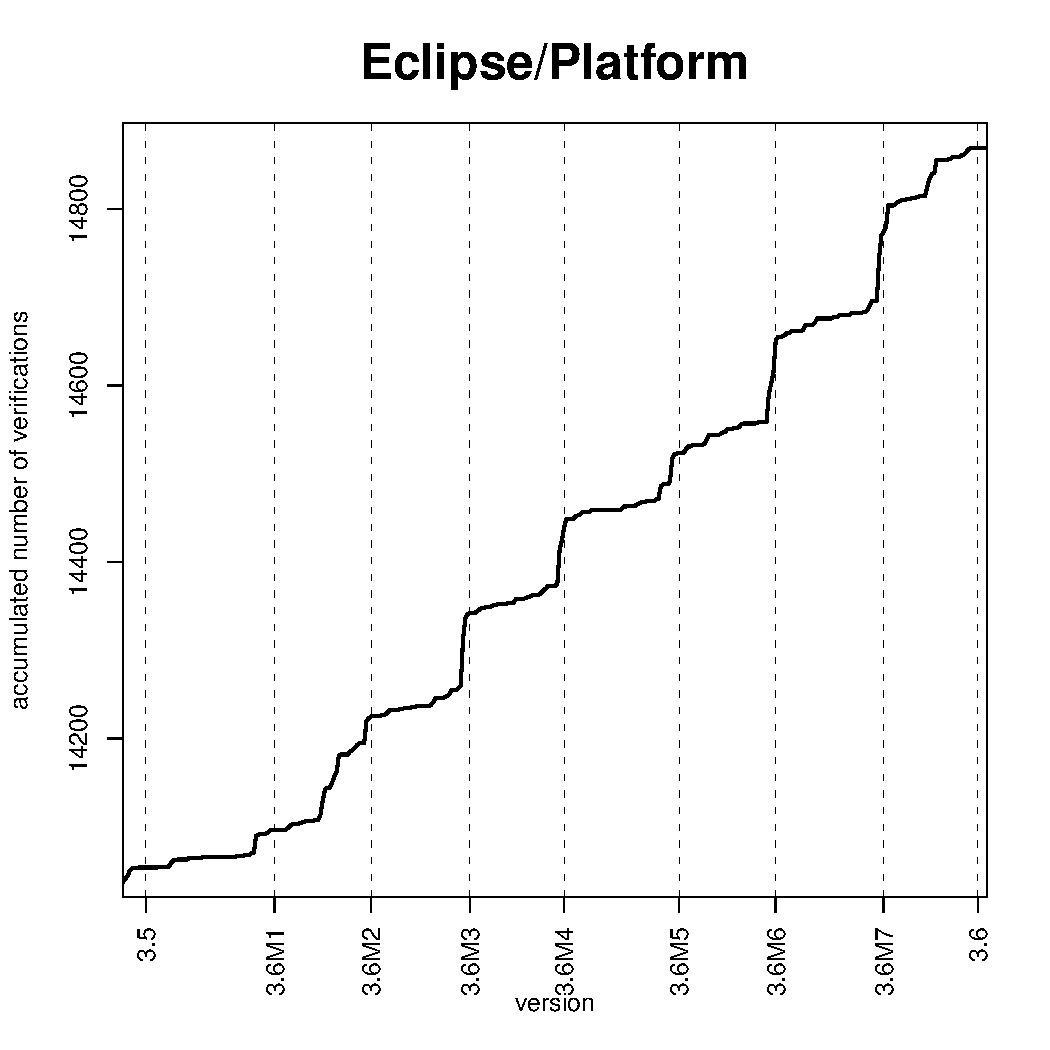
\includegraphics[width=0.25\textwidth]{milestones}}%\quad
\subfigure{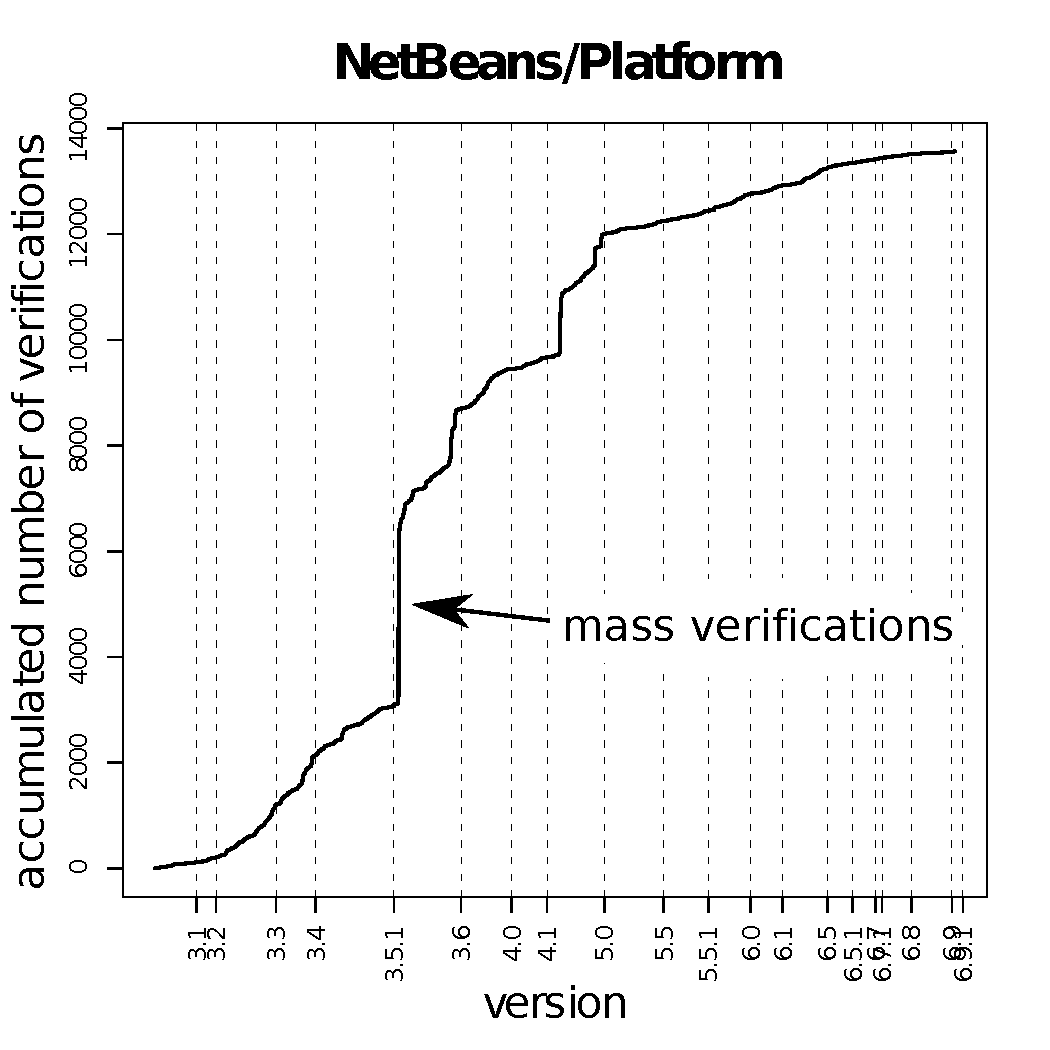
\includegraphics[width=0.25\textwidth]{cliffs} }}
\caption{Number of verifications over time.} \label{fig:when}
\end{figure}

% \begin{figure}[htbp]
% 	\centering
% 		\includegraphics[scale=1]{file}
% 	\caption{caption}
% 	\label{fig:label}
% \end{figure}

	For Eclipse/Platform, the graph shows the period between releases 3.5 and 3.6, including milestone releases every 6 or 7 weeks. It is clear from the graph that the verification activity is intensified in a few days preceding a milestone, represented in the graph by steeper ascents before the vertical lines. This pattern is an indicator of a verification phase. No such pattern was found in the other subprojects by analyzing their graphs (not shown here for brevity).

	The graph for NetBeans/Platform (Figure \ref{fig:when}, right side) shows the entire project history. Although there are steeper ascents, they are different because they do not precede release dates. Also, at a closer look, they represent thousands of verifications performed in a few minutes by the same developer, with the same comment. The same pattern was found in Eclipse/EMF (not shown).
	
	Of course, no developer can verify so many fixes in so little time. The explanation, supported by the comments, is that such mass verifications represent some cleanup of the bug repository, by marking old bugs as \VERIFIED---with no verification being actually performed. Researchers should take extra care with mass verifications, as they contain a large amount of bugs and, thus, are likely to bias the results of analyses.
	
	% 
	% We found evidence of a verification phase for Eclipse/Platform. In this project, verifications appear to be performed in bursts, with periods of intense activity separated by about 6 to 7 weeks of low or no activity. By taking a closer look in the period between the releases 3.5 and 3.6 (Figure XXX), it is clear that the periods of intense verification activity occur just before the milestones leading to 3.6.
	% 
	% No such pattern was found for NetBeans' subprojects.
	
	% We did not find evidence of a verification phase preceding each release. Unlike the bug fixing activity, the pace of verification is not steady, either. Instead, verification appears to be performed in bursts, which a couple of weeks with low or no activity, followed by a couple of days of intense verification activity.
	
	% In Eclipse, milestones are roughly 6 weeks apart from each other. Milestones are considered good enough for end users\footenote{\url{http://eclipsecon.org/2005/presentations/econ2005-eclipse-way.pdf}} The milestones are, in general, marked by a steep accent in verification just before the milestone date.
	% Weekly integration builds. Nightly builds. Build quality verified by automatic unit tests. 20k unit tests.
	
	%%%%%%%%%%%%%%%%%%%%%%
	
	% The first thing that comes to attention are ``cliff walls'', points in time when a large amount of bugs are verified, represented by steep, almost vertical portions of the plotted line. They appear in Eclipse/EMF and NetBeans/Platform. In NetBeans/Platform, all verifications in the cliff wall preceding version 5.5 share the same message: ``Verification of old issues''. For Eclipse/EMF, the message is ``Move to verified as per bug 206558'', which refers to the task of changing bugs marked as \FIXED\ to \VERIFIED.
	% 
	% Cliff walls represent a change in the development process, and the mass verification is needed in order to leverage useful features from Bugzilla (e.g., looking for verified bugs in order to aid the writing of release notes).
	
	% Because of cliff walls, extra care must be taken before doing any analysis that relies on the \VERIFIED\ status. In such situations, the \VERIFIED\ status is applied blindly, with no software verification being actually performed. Because cliff walls contain a large amount of bugs, they are likely to bias the results of analyses.
	
	%%%%%%%%%%%%%%%%%%%%%%
	
	% Some projects have ``cliff walls'' [reference graphic]. Taking a closer look, the VERIFIED status was used sparingly in Eclipse/EMF, but, suddenly, a huge number of bugs is verified and, after that, bugs tend to be verified frequently. It represents a change in the development process, and the mass verification is needed in order to leverage useful features from Bugzilla (e.g., looking for verified bugs in order to aid the writing of release notes).
	
	% If one is to build a predictive model based on verifications, the cliff walls should be ignored, as they represent unusual activity that has no connection with software verification whatsoever.
	
	% By visualizing release dates, we tried to assess if there is such a thing as a ``verification phase'', i.e., if verifications are frequent only on a period before the release. There was no evidence of such phase on Eclipse subprojects (TODO: look for patterns in NetBeans).
	
	% However, we found also that, different to what occur with fixes, verifications are not steady, constant. In Eclipse/Platform, for instance, there are periods of 3 to 5 weeks of few verifications, followed by a couple of days with intense verification activity (``mini cliff walls'', if you wish...)
	% 
	% The verifications of NetBeans/versioncontrol are more steady, continuous. Also, they seem to reflect well the FIXED curve.
	
	% TODO (future): are verifications more common on mondays on netbeans-versioncontrol?
	
	% TODO (future): how much time does it take between RESOLVED (FIXED) and VERIFIED?
	
\end{subsection}

\begin{subsection}{Who Verifies Bugs?}

	Table \ref{tab:qa} presents, for each subproject, the number of developers attributed to a QA team (i.e., developers who perform verifications at least 10 times more often than contribute bug fixes), and the proportion of bug verifications they account for.
	\newcommand\MyHead[2]{%
	  \multicolumn{1}{l}{\parbox{#1}{\centering #2}}
	}
	
	\begin{table}
		\begin{center}
		
		\caption{Discovered QA team for all four subprojects.}
		\begin{tabular}{l|r|r}
			% \toprule
			\textbf{\centering Project} & 
			\textbf{\centering QA team size} & 
			\MyHead{2.5cm}{\textbf{\% of verifications by QA team}} \\
			\hline
			Eclipse/Platform        & 4 (2.4\%)  &  1.1\% \\
			Eclipse/EMF             & 0 (0.0\%)  &  0.0\% \\
			NetBeans/Platform       & 5 (21.7\%) & 93.3\% \\
			NetBeans/VersionControl & 5 (20.8\%) & 93.2\% \\
			% \bottomrule
		\end{tabular}
		\end{center}

		\label{tab:qa}
	\end{table}
	
	% We counted the number of times each developer verified or fixed a bug. We consider that, if a developer is primarily concerned with quality assurance, then s/he verifies much more bugs that s/he fixes.
	% 
	% We defined ratio as ...
	% 
	% The verified/fixed ratio for the four projects is shown on Table XXX.
	
% \begin{verbatim}
% *** eclipse-platform 
% Verifiers: 4 (2.4%)
%   1.1% of verifications
% Fixers: 30 (17.9%)
% Total developers: 168 
% 
% *** eclipse-emf 
% Verifiers: 0 (0.0%)
%   0.0% of verifications
% Fixers: 4 (30.8%)
% Total developers: 13 
% 
% *** netbeans-platform 
% Verifiers: 5 (21.7%)
%   93.3% of verifications
% Fixers: 6 (26.1%)
% Total developers: 23 
% 
% *** netbeans-versioncontrol 
% Verifiers: 5 (20.8%)
%   93.2% of verifications
% Fixers: 6 (25.0%)
% Total developers: 24 
% \end{verbatim}
	
	In both NetBeans subprojects it is possible to infer the existence of a QA team, composed by approximately 20\% of the developers, that performs about 90\% of all verifications. In the Eclipse subprojects, there is no evidence of a dedicated QA team. In Eclipse/EMF no developer focus specifically on verification. In Eclipse/Platform, 2.4\% of the developers focus on verification tasks, contributing only to 1.1\% of the verifications.
	
% (it should be remembered that verification in EMF has a peculiar meaning)	
	
\end{subsection}

\end{section}

\begin{section}{Conclusion} \label{sec:conclusion}
	By analyzing four subprojects (two from Eclipse, two from NetBeans), we have found, using only data from bug repositories, subprojects with and without QA teams, with and without a well-defined verification phase. We also have found weaker evidence of the application of automated testing and source code inspection. Also, we have found cases in which marking a bug as \VERIFIED\ does not imply that any kind of software verification was actually performed.
			
	With the knowledge obtained from this exploratory research, we aim to improve and extend our previous work on the impact of independent verification on software quality. We can investigate, for example, whether verification performed by QA team is more effective than verification performed by other developers.
	
	Researchers should be aware that information about verification techniques may not be common in bug repositories, and that reported verification does not always correspond to actual verification. Some exploration of the data is important to avoid such pitfalls.
	
	% \begin{itemize}
	% 	\item Does independent verification improve software quality when it is performed by developers from the QA team?
	% 	\item Does independent verification improve software quality when it is performed as an separate phase of the software release cycle?
	% 	\item Does independent verification improve software quality when a particular verification technique (e.g., inspections, unit testing) is used?
	% \end{itemize}
	
\end{section}

\section*{Acknowledgment}

The first author is supported by FAPESB under grant BOL0119/2010.


% \section{Introduction}
% % no \IEEEPARstart
% This demo file is intended to serve as a ``starter file''
% for IEEE conference papers produced under \LaTeX\ using
% IEEEtran.cls version 1.7 and later.
% 
% All manuscripts must be in English. These guidelines include complete descriptions of the fonts, spacing, and related information for producing your proceedings manuscripts. Please follow them and if you have any questions, direct them to the production editor in charge of your proceedings at Conference Publishing Services (CPS): Phone +1 (714) 821-8380 or Fax +1 (714) 761-1784.
% % You must have at least 2 lines in the paragraph with the drop letter
% % (should never be an issue)
% 
% \subsection{Subsection Heading Here}
% Subsection text here.
% 
% 
% \subsubsection{Subsubsection Heading Here}
% Subsubsection text here.
% 
% \section{Type style and Fonts}
% Wherever Times is specified, Times Roman or Times New Roman may be used. If neither is available on your system, please use the font closest in appearance to Times. Avoid using bit-mapped fonts if possible. True-Type 1 or Open Type fonts are preferred. Please embed symbol fonts, as well, for math, etc.


% An example of a floating figure using the graphicx package.
% Note that \label must occur AFTER (or within) \caption.
% For figures, \caption should occur after the \includegraphics.
% Note that IEEEtran v1.7 and later has special internal code that
% is designed to preserve the operation of \label within \caption
% even when the captionsoff option is in effect. However, because
% of issues like this, it may be the safest practice to put all your
% \label just after \caption rather than within \caption{}.
%
% Reminder: the "draftcls" or "draftclsnofoot", not "draft", class
% option should be used if it is desired that the figures are to be
% displayed while in draft mode.
%
%\begin{figure}[!t]
%\centering
%\includegraphics[width=2.5in]{myfigure}
% where an .eps filename suffix will be assumed under latex, 
% and a .pdf suffix will be assumed for pdflatex; or what has been declared
% via \DeclareGraphicsExtensions.
%\caption{Simulation Results}
%\label{fig_sim}
%\end{figure}

% Note that IEEE typically puts floats only at the top, even when this
% results in a large percentage of a column being occupied by floats.


% An example of a double column floating figure using two subfigures.
% (The subfig.sty package must be loaded for this to work.)
% The subfigure \label commands are set within each subfloat command, the
% \label for the overall figure must come after \caption.
% \hfil must be used as a separator to get equal spacing.
% The subfigure.sty package works much the same way, except \subfigure is
% used instead of \subfloat.
%
%\begin{figure*}[!t]
%\centerline{\subfloat[Case I]\includegraphics[width=2.5in]{subfigcase1}%
%\label{fig_first_case}}
%\hfil
%\subfloat[Case II]{\includegraphics[width=2.5in]{subfigcase2}%
%\label{fig_second_case}}}
%\caption{Simulation results}
%\label{fig_sim}
%\end{figure*}
%
% Note that often IEEE papers with subfigures do not employ subfigure
% captions (using the optional argument to \subfloat), but instead will
% reference/describe all of them (a), (b), etc., within the main caption.


% An example of a floating table. Note that, for IEEE style tables, the 
% \caption command should come BEFORE the table. Table text will default to
% \footnotesize as IEEE normally uses this smaller font for tables.
% The \label must come after \caption as always.
%
%\begin{table}[!t]
%% increase table row spacing, adjust to taste
%\renewcommand{\arraystretch}{1.3}
% if using array.sty, it might be a good idea to tweak the value of
% \extrarowheight as needed to properly center the text within the cells
%\caption{An Example of a Table}
%\label{table_example}
%\centering
%% Some packages, such as MDW tools, offer better commands for making tables
%% than the plain LaTeX2e tabular which is used here.
%\begin{tabular}{|c||c|}
%\hline
%One & Two\\
%\hline
%Three & Four\\
%\hline
%\end{tabular}
%\end{table}


% Note that IEEE does not put floats in the very first column - or typically
% anywhere on the first page for that matter. Also, in-text middle ("here")
% positioning is not used. Most IEEE journals/conferences use top floats
% exclusively. Note that, LaTeX2e, unlike IEEE journals/conferences, places
% footnotes above bottom floats. This can be corrected via the \fnbelowfloat
% command of the stfloats package.



% \section{Conclusion}
% The conclusion goes here. this is more of the conclusion
% 
% % conference papers do not normally have an appendix
% 
% 
% % use section* for acknowledgement
% \section*{Acknowledgment}
% 
% 
% The authors would like to thank...
% more thanks here


% trigger a \newpage just before the given reference
% number - used to balance the columns on the last page
% adjust value as needed - may need to be readjusted if
% the document is modified later
%\IEEEtriggeratref{8}
% The "triggered" command can be changed if desired:
%\IEEEtriggercmd{\enlargethispage{-5in}}

% references section

% can use a bibliography generated by BibTeX as a .bbl file
% BibTeX documentation can be easily obtained at:
% http://www.ctan.org/tex-archive/biblio/bibtex/contrib/doc/
% The IEEEtran BibTeX style support page is at:
% http://www.michaelshell.org/tex/ieeetran/bibtex/
\bibliographystyle{IEEEtran}
% argument is your BibTeX string definitions and bibliography database(s)
\bibliography{IEEEabrv,msr2012-exploratory}
%
% <OR> manually copy in the resultant .bbl file
% set second argument of \begin to the number of references
% (used to reserve space for the reference number labels box)
% \begin{thebibliography}{1}
% 
% \bibitem{IEEEhowto:kopka}
% H.~Kopka and P.~W. Daly, \emph{A Guide to \LaTeX}, 3rd~ed.\hskip 1em plus
%   0.5em minus 0.4em\relax Harlow, England: Addison-Wesley, 1999.
% 
% \end{thebibliography}




% that's all folks
\end{document}


